% Diagrama de clases
\newcommand{\clases}{

\begin{tikzpicture}
\tikzumlset{fill class=white, font=\tiny}
% Clase Pizarra
\umlclass[x=-6, y=5]{Pizarra}{
  -- estado : Estado \\ 
  -- usuarios : Vector$<$Usuario$>$\\
  -- estadisticas : Vector$<$Estadisticas$>$\\
  -- niveles : Vector$<$Nivel$>$\\
  -- conf : Configuracion\\
}{ 
  + mostrarEstadisticas(String userid, Usuario user):String\\
  + mostrarEstadisticasGenerales(Usuario user):String\\
  + escribir(String direccion, Archivo archivo, Usuario user)\\
  + leer(String direccion, Usuario user):Archivo\\
  + escrituraLectura(String direccion, Archivo archivo, Usuario user): Archivo\\
  + mostrarEstado(Usuario user):Usuario\\
  + buscar(String nombre, Usuario user):Estado\\
  + comparar(Archivo arch1, Archivo arch2, Usuario user):Archivo\\
  + crearCarpeta(String direccion, String nombre, Usuario user): Bool\\
  + crearUsuario(String nombre, String userid, String pass, Nivel nivel, Usuario user)\\
  + gestionarPermisos(Nivel nivel, Bool[] permisos, Usuario user): Bool\\
  + configurarPizarra(Configuracion config, Usuario user): Bool\\
  + getUsuario(String userid):Usuario\\
  -- setEstado(Estado)\\
  -- setUsuarios(Vector$<$Usuario$>$)\\
  -- setEstadisticas(Vector$<$Estadisticas$>$)\\
  -- comprobarPermisos(Usuario user, int permiso):Bool
}

% Clase Agente
\umlclass[x=-6, y=-2.5]{Agente}{
  -- userid : String\\
  -- pass : String\\
  -- pizarra : Pizarra\\
  -- usuario : Usuario\\
}{
  + Agente(String userid)\\
  + Agente(Pizarra pizarra)\\
  + iniciarSesion(String userid, String pass):Bool\\
  + mostrarEstadisticas(String userid)\\
  + mostrarEstadisticasGenerales()\\
  + escribir(String direccion, Archivo archivo)\\
  + leer(String direccion):Archivo\\
  + escrituraLectura(String direccion, Archivo archivo):Archivo\\
  + mostrarEstado():Estado\\
  + buscar(String nombre):String\\
  + comparar(Archivo arch1, Archivo arch2):Archivo\\
  + crearCarpeta(String direccion, String nombre):Bool\\
  + crearUsuario(String nombre, String userid, String pass, Nivel nivel)\\
  + gestionarPermisos(Nivel nivel, Bool[] permisos): Bool\\
  + configurarPizarra(Configuracion config)\\
  + setUserid(String userid)\\
  + setPass(String pass)\\
  -- comprobarPermisos(Usuario user, int permiso):Bool\\
  -- establecerConexion(Pizarra pizarra)\\
  -- cerrarSesion(Pizarra pizarra) 
}

% Clase Usuario
\umlclass[x=2, y=-1]{Usuario}{
  -- nombre : String\\
  -- userid : String\\
  -- pass : String\\
  -- nivel : Nivel
}{
  + comprobarUser(String pass): Bool\\
  + getNombre() : String\\
  + getUserid() : String\\
  + getNivel() : Nivel\\
  + setPass(String pass)\\
  + setNivel(Nivel nivel) 
}

% Clase Estadisticas
\umlclass[x=2, y=3]{Estadisticas}{
  -- userid : String\\
  -- datos[] : Integer\\
}{
  + actualizarEstadisticas(datos[] int)\\
  + getUsuario() : String\\
  + getDatos() : Integer[]\\
}

% Clase Configuracion
\umlclass[x=2, y=9.5]{Configuracion}{
  -- visibilidad : Bool\\
  -- IP : String\\
  -- puerto : int\\
  -- maxConexion : int\\
  -- espacio : int\\
  -- maxUser : int\\
  -- depuracion : Bool\\
}{
}

% Clase Estado
\umlclass[x=-9, y=10]{Estado}{
  -- Vector$<$Elemento$>$
}{

}

% Clase Elemento
\umlclass[x=-16, y=10]{Elemento}{
   \# nombre : String
}{

}

% Clase Carpeta
\umlclass[x=-18, y=6]{Carpeta}{
   -- Vector$<$Elemento$>$
}{

}

% Clase Archivo
\umlclass[x=-13, y=7]{Archivo}{

}{

}

% Clase Nivel
\umlclass[x=-16, y=3]{Nivel}{
   -- permisos[\$NPermisos\$] : Bool
}{
   + cambiarPermiso(int permiso, estado Bool)\\
   + resetPermisos()\\
   + setPermisos()\\
   + getPermisos():Bool[]
}

% Relaciones

\umlinherit[geometry=-|]{Carpeta}{Elemento}

\umlcompo[mult1=0..n, mult2=1]{Elemento}{Carpeta}

\umlinherit{Archivo}{Elemento}

\umlcompo[mult2=1, mult1=0..n]{Elemento}{Estado}

\umlimpl{Pizarra}{Nivel}

\umlimpl[geometry=-|]{Pizarra}{Estado}

\umlimpl{Pizarra}{Configuracion}

\umlimpl{Pizarra}{Estadisticas}

\umlimpl{Pizarra}{Usuario}

\umlimpl{Agente}{Pizarra}

\end{tikzpicture}

}

\newcommand{\clasesanalisis}{

\begin{tikzpicture}
\tikzumlset{fill class=white}
% Clase Pizarra
\umlclass[x=-6, y=5]{Pizarra}{
  -- estado : Estado \\ 
  -- usuarios : Vector$<$Usuario$>$\\
  -- estadisticas : Vector$<$Estadisticas$>$\\
  -- niveles : Vector$<$Nivel$>$\\
  -- conf : Configuracion\\
}{}

% Clase Agente
\umlclass[x=-6, y=-2.5]{Agente}{
  -- userid : String\\
  -- pass : String\\
  -- pizarra : Pizarra\\
  -- usuario : Usuario\\
}{}

% Clase Usuario
\umlclass[x=2, y=-1]{Usuario}{
  -- nombre : String\\
  -- userid : String\\
  -- pass : String\\
  -- nivel : Nivel
}{}

% Clase Estadisticas
\umlclass[x=2, y=3]{Estadisticas}{
  -- userid : String\\
  -- datos[] : Integer\\
}{}

% Clase Configuracion
\umlclass[x=2, y=9.5]{Configuracion}{
  -- visibilidad : Bool\\
  -- ip : IP\\
  -- puerto : int\\
  -- maxConexion : int\\
  -- espacio : int\\
  -- maxUser : int\\
  -- depuracion : Bool\\
}{}

% Clase Estado
\umlclass[x=-9, y=10]{Estado}{
  -- Vector$<$Elemento$>$
}{}

% Clase Elemento
\umlclass[x=-16, y=10]{Elemento}{
   \# nombre : String
}{}

% Clase Carpeta
\umlclass[x=-18, y=6]{Carpeta}{
   -- Vector$<$Elemento$>$
}{}

% Clase Archivo
\umlclass[x=-13, y=7]{Archivo}{

}{}

% Clase Nivel
\umlclass[x=-16, y=-2]{Nivel}{
   -- permisos[] : Bool
}{}



% Relaciones

\umlinherit[geometry=-|]{Carpeta}{Elemento}

\umlcompo[mult1=0..n, mult2=1]{Elemento}{Carpeta}

\umlinherit{Archivo}{Elemento}

\umlcompo[mult2=1, mult1=0..n]{Elemento}{Estado}

\umlimpl{Pizarra}{Nivel}

\umlimpl[geometry=-|]{Pizarra}{Estado}

\umlimpl{Pizarra}{Configuracion}

\umlimpl{Pizarra}{Estadisticas}

\umlimpl{Pizarra}{Usuario}

\umlimpl{Agente}{Pizarra}

\end{tikzpicture}

}